\documentclass[a4paper,12pt]{scrartcl}
\usepackage[utf8]{inputenc}
\usepackage[UKenglish]{isodate}
\usepackage{csquotes}
\usepackage{graphicx}
\usepackage{wrapfig}
\usepackage{enumitem}
\usepackage{pdflscape}
\usepackage[toc,page]{appendix}
\usepackage{geometry}
\usepackage{hyperref}
\usepackage{cleveref}
\usepackage{listings}
\usepackage{csvsimple}
\usepackage{booktabs}
\usepackage{longtable}
\usepackage{caption}
\usepackage{subcaption}
\usepackage[colorinlistoftodos]{todonotes}
\usepackage[british]{babel}
\usepackage{float}
%\usepackage[margin=1in]{geometry}
\usepackage{listings}
\usepackage{color}
 
\definecolor{codegreen}{rgb}{0,0.6,0}
\definecolor{codegray}{rgb}{0.5,0.5,0.5}
\definecolor{codepurple}{rgb}{0.58,0,0.82}
\definecolor{backcolour}{rgb}{0.95,0.95,0.92}
 
\lstdefinestyle{mystyle}{
	language=PHP,
    backgroundcolor=\color{backcolour},   
    commentstyle=\color{codegray},
    keywordstyle=\color{magenta},
    numberstyle=\tiny\color{codegray},
    stringstyle=\color{codegreen},
    basicstyle=\footnotesize,
    breakatwhitespace=false,         
    breaklines=true,                 
    captionpos=b,                    
    keepspaces=true,                 
    numbers=left,                    
    numbersep=5pt,                  
    showspaces=false,                
    showstringspaces=false,
    showtabs=false,                  
    tabsize=3,
    morekeywords={ new, __halt_compiler, abstract, and, array, as, break, callable, case, catch, class, clone, const, continue, declare, default, die, do, echo, else, elseif, empty, enddeclare, endfor, endforeach, endif, endswitch, endwhile, eval, exit, extends, final, for, foreach, function, global, goto, if, implements, include, include_once, instanceof, insteadof, interface, isset, list, namespace, new, or, print, private, protected, public, require, require_once, return, static, switch, throw, trait, try, unset, use, var, while, xor}
}

\lstset{language=Java,
  showspaces=false,
  showtabs=false,
  breaklines=true,
  showstringspaces=false,
  breakatwhitespace=true,
  commentstyle=\color{pgreen},
  keywordstyle=\color{pblue},
  stringstyle=\color{pred},
  basicstyle=\ttfamily,
  moredelim=[il][\textcolor{pgrey}]{$$},
  moredelim=[is][\textcolor{pgrey}]{\%\%}{\%\%}
}
 
\lstset{style=mystyle}

\graphicspath{ {images/} }
\usepackage[
	backend=biber,
	style=ieee,
	]{biblatex}

\addbibresource{references.bib}

\title{Case study of A National Programme for IT with regards to Managing Software Intensive Projects}
\author{James Fernando}
\date{\today}

\begin{document}
	
	\begin{titlepage}
		\maketitle
	\end{titlepage}
	
	\tableofcontents
	\newpage
	\section{Introduction}
	{
		
	}
	\section{Project Background}
	{
		NHS Connection for health is a section of the Department of Health which was in charge of producing a national programme for IT to allow for the sharing of patient information, this was set up in 2005\cite{nhsconnectingforhealth2019}. However some of the ideas for centralising patient information had been published in 1998. The quote below lists a couple of the ideas listed in a book published by the Department for Health in 1998.
		\begin{displayquote}{frankburns1998}
			\label{qoute:ConnectingForHealthPlans}
			individualised personal electronic records will be developed to provide NHS
			professionals with 24 hour secure access to the information important to
			individual patients’ care, when required. This will immeasurably improve
			emergency care and ensure any professional involved in the care of an
			individual is up to date with their treatment
			
			on-line services will be provided for GPs and their patients, to make hospital
			appointments as required or diagnostic results when due. The sight of hard
			pressed NHS professionals rummaging about in buff folders or hand-writing
			referrals and test requests will be consigned to history as soon as possible.
		\end{displayquote}
	}
	\section{Project Goal}
	{
		The national program for It was supposed to make use of technology to allow for easier and better sharing of patient information and medical information. Some of the systems and services has been listed below:
		\begin{displaycquote}{nhsconnectingforhealth2019}
			\begin{itemize}
				\item {creating an NHS Care Records Service to improve the sharing of patients' records across the NHS with their consent}
				\item {making it easier and faster for GPs and other primary care staff to choose and book hospital appointments for patients}
				\item {generating, transmitting and dispensing electronic prescriptions}
				\item {ensuring that the IT infrastructure can meet NHS needs now and in the future}
				\item {allowing x-rays and scans to be captured, viewed and stored digitally}
				\item {enabling patients' electronic health records to be transferred directly when they move from one GP practice to another}
				\item {linking the NHS with a secure email and directory service}
			\end{itemize}
		\end{displaycquote}
	}
	\section{Project Type}
	{
		\subsection{NTCP Diamond}
		{
			\begin{figure}
				\centering
				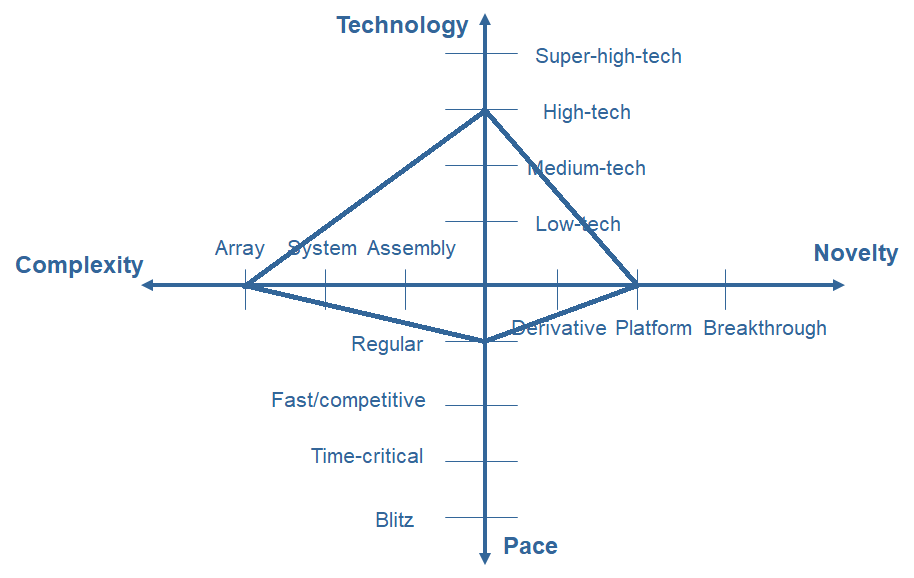
\includegraphics[width=\textwidth]{NationalProgrammeForITNTCP.png}
				\label{fig:NTCPDigram}
				\caption{Shows the NTCP Diamond created for the National Programme for IT project}
			\end{figure}
		}
	}
	\section{Project Success Measures}
	{
		
	}
	\section{Software/IT Challenge}
	{
		
	}
	\section{Rational vs Actual}
	{
		
	}
	\section{Maturity Model}
	{
		
	}	
	\section{Appropriate and Inappropriate Approaches}
	{
		
	}
	\section{User Participation}
	{
		
	}
	\section{Software Engineering}
	{
		
	}
	\section{Conclusion}
	{

	}
	
	
	\newpage
	
	\printbibliography[heading=bibintoc,title=References]
\end{document}
